\section{Scholarly Search And Ranking}   %Model
\label{sec-model}





In this section, we first introduce scholarly search, and then present the ranking model that lays its core foundation.


\subsection{Scholarly Search}
Our \oursystem system facilitates the research activities of scholars by providing four types of entity searches as follows.


\stitle{Article search}. Given a set of keywords, \oursystem returns a sorted list of  articles whose titles {\em contain} the given keywords. In the meantime, it also returns three sorted lists of authors, venues and affiliations associated with the returned articles.

%For each author (resp. venue and affiliation),  we combine the importance score of the author and the importance score of all articles of the author under the keywords. The same is true for affiliations and venues.

\stitle{Author, venue and affiliation searches}. Given a (partial) name of an author, venue or affiliation, \oursystem returns a sorted list of  authors, venues or affiliations, respectively, that {\em contain} the given (partial) name.




\subsection{Scholarly Article Ranking}
\label{subsec:rankingMetric}

\oursystem provides five metrics to support article search.


%Here, $S(v)$ is a static ranking score of article, $Q(j)$ is the j$th$ of query keywords vector which have removed stop words, $idf(Q_j)$ is inverse document frequency measures how much information the word $Q(j)$ provides, $T$ suggests we aggregate the title word vectors to their centroid and $\theta$ means the relevance factor.

\eat{%%%%%%%%%%%%%%%%
\begin{figure}[tb!]
\centering
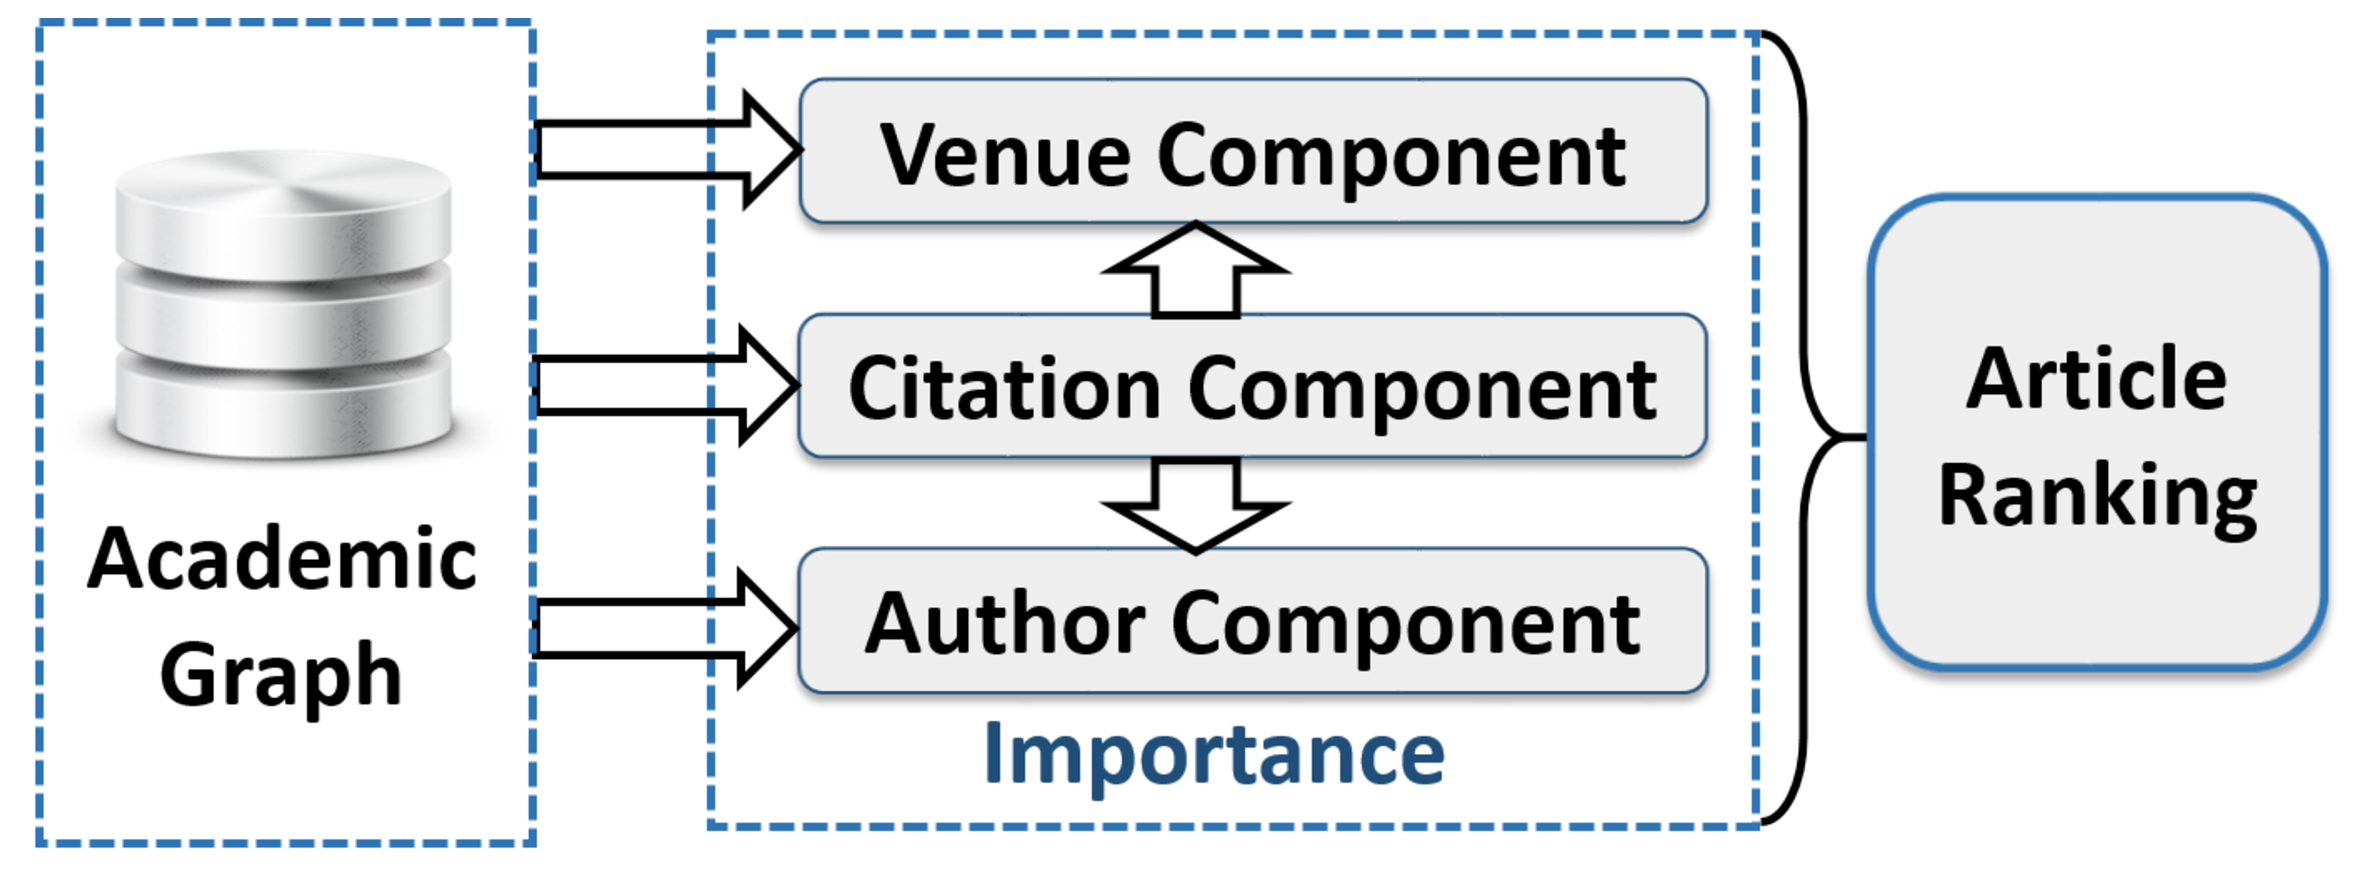
\includegraphics[scale=0.15]{framework-lite-2.eps}
%\vspace{-1ex}
\caption{\sarank framework~\cite{ma2018query}} \label{fig:sarank}
\vspace{-2ex}
\end{figure}
}%%%%%%%%%%EAT





\stitle{Citation counts and publish time}. Articles are simply sorted based on their citation counts and publish time. %, respectively, and ties are broken by further comparing importance scores.


\stitle{Importance}. This metric comes from our recently developed \sarank (please refer to~\cite{ma2018query} for details). The importance of an article is defined as a combination of its prestige and popularity, where prestige is computed by a novel Time-Weighted PageRank, and popularity is the sum of citation freshness. To assign newly published articles reasonable ranking scores, it further assembles the importance of citations, authors and venues to derive the final ranking. %, as illustrated in Fig.~\ref{fig:sarank}.

The above three are for {\em query independent ranking}, and we introduce another two metrics for {\em query dependent ranking}.

\stitle{Relevance}. This metric enables to rank scholarly articles in terms of the semantic correlation between their titles and given queries (keywords). Nowadays Word2vec \cite{corrado2013efficient} has become the {\em de facto} standard to capture semantics, and we  utilize Word2vec to evaluate semantic relevance as follows:
%
%\begin{equation}
%\label{eq:relscore}
%rel(a, Q) = \sum_{t \in a.T} \sum_{q \in Q} idf(q) \frac {\textbf{t} \cdot \textbf{q}} {|| \textbf{t} ||\ ||\textbf{q}||}.
%\end{equation}
%
\begin{equation}
\label{eq:relscore}
rel(a, Q) = \sum_{t \in a.T} \sum_{q \in Q} \frac {\textbf{t} \cdot \textbf{q}} {|| \textbf{t} ||\ ||\textbf{q}||}.
\end{equation}

Here $a.T$ and $Q$ are the sets of words (excluding stop words) in the title of an article $a$ and the query, respectively, %$idf(q)$ is the inverse document frequency of a word $q$,
and $\textbf{t}$ and $\textbf{q}$ are the corresponding embeddings of words $t$ and $q$.
%Although the entire article to compute the relevance can improves relevance accuracy, it is not the main concern of our work, we just briefly touch on this and will explore it in future work.
Note that the abstracts and full texts of scholarly articles may not \marked{be} available for scholarly systems, and word embeddings are pre-trained with external corpus.

% may not available for -> may not be available for 

%Note that the abstracts and full texts are not available for most scholarly articles in our data and word embeddings are pre-trained with external corpus.


\stitle{Relevant importance.} The previous importance metric does not consider the closeness of the articles with respect to given queries. This metric is to rank scholarly articles by combining the semantic relevance and importance metrics. More specifically, we first normalize the computed relevance (resp. importance) score by scaling with the maximum relevance (resp. importance) score in the resulting article set, and we then define the relevant importance score as follows.
\begin{equation}
\label{eq:relimp}
rImp(a, Q) = \alpha \cdot rel_n(a, Q) + (1-\alpha)\cdot imp_n(a),
\end{equation}
where $rel_n(a, Q)$ and $imp_n(a)$ are the {\em normalized} semantic relevance and importance scores, and $\alpha$ is a regularization parameter,
typically set to an empirical value in [0.2, 0.4].
% which is set to 0.2 in \oursystem.



%\subsection{Author, Venue and Affiliation Ranking}
\subsection{Author,Venue and Affiliation Ranking}
\label{subsec:heteroRanking}

For authors, venues and affiliations,  \oursystem provides stand-alone ranking and article-coupled ranking.

\stitle{Stand-alone ranking}. To support author, venue and affiliation searches, \oursystem ranks authors, venues and affiliations with the sum of the query independent ranking scores of all their associated articles. Further, when sorting entities by publish time, it uses an \marked{exponentially decayed score} $e^{T_a-T_0}$ to evaluate the research activeness of an entity, where $T_a$ is the publish year of an article $a$, and $T_0$ is the current year.

% exponentially decayed ranking score -> exponentially decayed score 

\stitle{Article-coupled ranking}. To support scholarly entity search, \oursystem ranks authors, venues, and affiliations \marked{regarding} the resulting articles of a specific scholarly entity query, along the same lines as stand-alone ranking. This helps to answer questions such as which authors, venues or affiliations are the most authoritative ones in the query related field of study.

% with respect to -> regarding


%To support article search, \oursystem ranks authors, venues, and affiliations with respect to the resulting articles of an article search query, along the same lines as stand-alone ranking. This helps to answer questions like which authors (venues or affiliations) are the most authoritative ones in the query related field of study.

The search and ranking functions of \oursystem and existing systems are summarized in Table~1.
%The search and ranking functions of \oursystem and existing systems are summarized in Table~1, where metrics are not reported due to their unavailability in commercial systems.



\eat{
-------------------- original version --------------------  \\
We first introduce Time-Weighted PageRank for evaluating the importance of entities, defined as a combination of the prestige and popularity, and then introduce entity ranking including author ranking, venue ranking, affiliation ranking and type ranking \itshape e.g., \upshape relevance ranking.


\subsection{Time-Weighted PageRank}
\par
PageRank is a typical method in scholarly articles ranking as we can easily make use of the reference between different articles. Due to the following reasons: (1) Different articles typically have different impacts in practice, and there is a need to differentiate, while PageRank essentially assumes equal impacts (2) The semantics of citation relationships are time-dependent, which means that citations at different periods of time may reveal different information. We introduce Time-Weighted PageRank(TWPageRank) by extending a time decay factor because of the impact of an article decay with time after peak time.
% why time weight pagerank

\par
We present TWPageRank that evaluate the prestige of nodes in a directed graph, in which each node attached with time information. And we use \itshape the impact weight \upshape to describe the relative weight from the edge sources to targets. Formally, the impact weight on a directed edge $(u,v), i.e.,$ an edge $u$ from $v$, is defined as:

\begin{equation}
\centering
\label{eq:edgeWeight}
w(u,v)=\left \{
\begin{array}{ccl}
1                        &    &{T_u   <   Peak_v} \\
e^{\sigma (T_u-Peak_v)}  &    &{T_u   \ge Peak_v} \\
\end{array} \right.
\end {equation}
where $T_u$ is the time of node $u$, $Peak_v$ is the peak time of node $v$ after which the impact weights of edges to $v$ decay with time, and $\sigma$ is a negative number controlling the decaying speed of the impacts. By default, we use years as its time granularity in Eq. (\ref{eq:edgeWeight}).

\par
Thus, the update rule of Time-weighted PageRank is

\begin{equation}
\centering
\label{eq:twPR}
PR(v)= d \sum_{(u,v)\in E} \frac{w(u,v)PR(u)}{W(u)} + \frac{1-d}{n}
\end{equation}
where $PR(u)$ and $PR(v)$ are the TWPageRank score of $u$ and $v$. And $E$ is a set of edges, $W(u)=\sum_v w(u,v)$ is the sum of the impact weights on all edges from $u$, $n$ is the number of nodes and $d$ is a damping parameter in (0, 1).
% what's TWpagerank


\subsection{Entity Ranking and Type Ranking}
\par
Scholarly entities(\itshape e.g., \upshape affiliation, venue, author and article) ranking is a problem of assessing the importance of nodes in a heterogeneous network. The importance is a combination of \itshape prestige \upshape and \itshape popularity \upshape to capture the evolving nature of entities. The prestige of scholarly entities is derived by applying TWPageRank on the citation graph $G$, and each type of entity is assigned the corresponding TWPageRank score as its prestige score $Prs$.

\par
To learn about the popularity of different scholarly entities, we first introduce the popularity of an article. The popularity of an article $v$ is the sum of all its citation freshness, \itshape i.e., \upshape the closeness to the current year:
\begin{equation}
\centering
\label{eq:pop}
Pop (v) = \sum_{(u,v) \in E^c} e^{\sigma(T_0 - T_u)}
\end{equation}
Here, $T_0$ is the current year, $T_u$ is the largest year among all articles, $\sigma$ is the negative decaying factor in Eq. (\ref{eq:edgeWeight}).

\par
Intuitively, prestige favors those with many citations soon after the publication of articles or associated articles of venues and authors, and popularity capture the temporal nature of entities.


\textbf{Affiliation Ranking.} We computes the importance of affiliations by their associated articles. As the importance of an affiliation evolves with time, we treat the affiliation importance in each year individually, and its importance is the sum of importance in all individual years.

\par
We construct an affiliation graph $G^a(V^a, E^a)$ using the citation information among affiliations, in which a node represents an affiliation in a specific year and a direct edge $(s, t)$  means that there exists articles of affiliation $s$ citing articles of affiliation $t$. Thus, the impact weights are defined as sums of impact weights from affiliation $s$ to affiliation $t$, \itshape i.e., \upshape
\begin{equation}
\centering
\label{eq:authorSumWeight}
w_a(s,t) = \sum_{u \in C(s), v \in C(t)} w(u,v)
\end{equation}
Here, $C(s)$ and $C(t)$ are the sets of articles of affiliation $s$ and affiliation $t$, and $w(u,v)$ is the impact weight of articles $u$ and $v$.
% define the impact weight between between author s and author t

\par
The prestige of an affiliation in a specific year ($Prs_a$) is computed using the impact weights Eq. (\ref{eq:authorSumWeight}) and the update rule in Eq. (\ref{eq:twPR}). The popularity of an affiliation in a specific year ($Pop_a$) is defined as the average popularity of its articles that is computed using Eq. (\ref{eq:pop}). Thus, the \itshape affiliation importance score \upshape ($Imp_a$) is defined as a combination of its prestige and popularity:
\begin{equation}
\centering
\label{eq:imp}
Imp_a(v) = Prs_a(v)^{\lambda} Pop_a(v)^{1-\lambda}
\end{equation}
Here, $\lambda \in [0, 1]$ is the importance factor, indicates the weighting about prestige and popularity.

\textbf{Venue Ranking.}
We computes the importance of venue using their associated articles which is similar with affiliation ranking. We treat the venue importance in each year, and construct a venue graph $G^v(V^v, E^v)$ using citation information among venues. And then we combine the prestige of a venue ($Prs_v$) and the popularity of venue ($Pop_v$) as the \itshape venue importance score \upshape ($Imp_v$).


\textbf{Author Ranking.}
We evaluate the importance of each author, and compute the average importance of the authors of an article as its \itshape author importance score. \upshape However, it is obvious that the author citation graph is too large to handle. Hence, we evaluate the prestige, popularity of the author by using the average prestige, popularity of all her/his published articles, respectively. Then, the author importance score ($Imp_{aut}$) is the combination of its prestige and popularity, similar to affiliation ranking.


\textbf{Article Ranking.}
If we are only to rank scholarly articles, the other type of entities such as venues and authors are closely involved. Hence, we assemble the importance of article, venue and author to produce the final scholarly articles ranking, illustrated in Fig. 1. Venue ranking and author ranking have presented in previous paragraphs. Next, introduce how to compute the importance of article using citation information.

\par
We first construct a citation graph $G^c(V^c, E^c)$ using citation information among articles. The prestige of articles ($Prs_c$) is derived by using TWPageRank in citation graph $G^c$. The popularity of an article ($Pop_c$)is the sum of all its freshness which has described in Eq. (\ref{eq:pop}). The importance of citation component ($Imp_c$) is a combination of its prestige and popularity in the citation graph by applying Eq. (\ref{eq:imp}).

\par
Thus, the static ranking score of an article $v$ is aggregated as follows:
\begin{equation}
\centering
\label{eq:assemble}
S(v) = \alpha Imp_v(v) + \beta Imp_{aut}(v) + (1 - \alpha - \beta)Imp_c(v)
\end{equation}
Here parameter $\alpha$, $\beta$ and $1- \alpha - \beta$  regularize the contributions of the venue, author and citation information.


\textbf{Relevance Ranking.} We have introduced affiliation, venue, author, article ranking in the former sections. These rankings are query independent and
aim to give a static ranking based on scholarly data only. However, it is vital to evaluate the similarity between the short query and sentence (\itshape i.e., \upshape title of the paper) when retrieve articles by keywords.

\par
Hence, we employ distributional semantic approach to represent words. Similarities between the term vectors indicates the corresponding semantic similarities \cite{corrado2013efficient}. The final ranking score of an article $v$ that relates to semantics of article title, defined as follow:
\begin{equation}
\centering
\label{eq:simscore}
F(v) = \theta S(v) + (1- \theta) \sum_j idf(Q_j) \frac {Q_j \cdot T} {\left \| Q_j \right \| \left \| T \right \|}
\end{equation}
Here, $S(v)$ is a static ranking score of article, $Q(j)$ is the j$th$ of query keywords vector which have removed stop words, $idf(Q_j)$ is inverse document frequency measures how much information the word $Q(j)$ provides, $T$ suggests we aggregate the title word vectors to their centroid and $\theta$ means the relevance factor.
} %%% end of \eat
